\newif\ifpublic
\publicfalse% This is the camera-ready MKM paper -> mkm09.pdf
%\publicfalse% This is the blue note

\ifpublic
\documentclass{llncs}
\else 
\documentclass[12pt]{scrartcl}
\fi 

% Draft?
\newif\ifdraft
%\drafttrue
\draftfalse

% \usepackage[english]{babel}
\usepackage[T1]{fontenc}
\usepackage[utf8]{inputenc}
\ifpublic\else
\usepackage{lmodern}
\fi
\usepackage{textcomp}
\usepackage{amstext}
\usepackage{ifthen}
\usepackage{graphicx}
\usepackage{paralist}

\ifdraft
\usepackage[show]{ed}
\usepackage{pdfsync}
\pagestyle{plain}
\usepackage[eso-foot,today]{svninfo}
\svnInfo $Id: note.tex 8487 2009-08-11 22:09:44Z clange $
\svnKeyword $HeadURL: https://svn.omdoc.org/repos/omdoc/trunk/doc/blue/foaf/note.tex $
\else
\ifpublic
\else
\usepackage[hide]{ed}
\usepackage{microtype}
\fi
\fi

\usepackage[hyper]{acronyms}
\usepackage{lstomdoc,xmlindex,myref}

% KWARC slides
\ifpublic
\else
\usepackage{home}
\fi

\usepackage{hyperref}
\lstset{language=[1.6]OMDoc,basicstyle=\scriptsize}
\lstset{columns=flexible}
\def\llquote#1{\ensuremath{\langle\kern-.25em\langle\hbox{\sl{#1}}\rangle\kern-.25em\rangle}}

\usepackage{xspace}
\renewcommand{\omdoc}{\textsc{OMDoc}\xspace}

%%%% to save space here. 
%\def\subsection#1{\medskip\goodbreak\refstepcounter{subsection}\textbf{\arabic{section}.\arabic{subsection} #1}}

\begin{document}

\title{A Mathematical Approach to Ontology Authoring and Documentation}
\ifpublic
\author{Christoph Lange and Michael Kohlhase}
\institute{Computer Science, Jacobs University, Bremen, Germany\\
  \email{\{ch.lange,m.kohlhase\}@jacobs-university.de}}
\else
\author{Christoph Lange, Michael Kohlhase\\
Computer Science\\
Jacobs University, Bremen}
\fi

\maketitle
\begin{abstract}
  The semantic web ontology languages RDFS and OWL are widely used but limited
  in both their expressivity and their support for modularity and integrated
  documentation.  Expressivity, modularity, and documentation of formal
  knowledge have always been important issues in the MKM community.  Therefore,
  we try to improve these ontology languages by well-tried MKM techniques.

  Concretely, we propose embedding the language concepts into \omdoc to make use of its
  modularity and documentation infrastructure. We show how \omdoc can be made compatible
  with semantic web ontology languages, focusing on knowledge representation, modular
  design, documentation, and metadata.  We evaluate our technology by re-implementing the
  Friend-of-a-friend (FOAF) ontology and applying it in a novel metadata framework for
  technical documents (including ontologies).
\end{abstract}

\section{Introduction}\label{sec:intro}

The concept of an ``ontology'' as a formalization of a shared conceptualization
\ifpublic\else\ednote{maybe cite Gruber, if we have space}\fi is at the heart of the
semantic web -- the web of data and intelligent agents.  RDFS (RDF Schema/Vocabulary
Description Language~\cite{BrGu04:rdfs}) and OWL (Web Ontology
Language~\cite{McGvHa:owl04}), the major semantic web ontology languages, have a limited
expressivity: The common OWL sublanguages OWL-Lite and OWL-DL implement two different
description logics -- decidable subsets of first-order logic~\cite{DL-handbook07}.  This
was a deliberate design goal as decidability is a prerequisite for web scalability.  A
common experience in ontology design is, however, that certain axioms in the domains to be
modeled exceed the expressivity of the languages chosen for implementation.  Sometimes,
dumbing down the model to less expressive special cases\footnote{as has, e.\,g., been done
  for the DOLCE ontology, a simplified version of which has been formalized in OWL-DL;
  cf.\ \url{http://www.loa-cnr.it/DOLCE.html}.} is sufficient, whereas in other cases, a
prose description of the actual axiom is added to the documentation of the ontology.

An example for the latter can be seen in the Friend-of-a-Friend (FOAF)
ontology~\cite{FOAF:spec} for modeling user profiles and simple social relationships:
Usually, a \textit{foaf:Group} has members of type \textit{foaf:Agent}, where an agent can
be a group, a person, or an organization.  The \textit{foaf:membership\-Class} property
can be used to be more specific about the type of the members of a group by linking an
instance of \textit{foaf:Group} to an RDFS or OWL \textit{Class}.  We can, e.\,g., require
that all members of the KWARC research group in Bremen be computer scientists.  Then, if
we state that Michael is a member of KWARC, we would like a reasoner to infer that he is a
computer scientist, or, vice versa, to complain, if he is classified as a type of person
that is not consistent with being one.  This combination of ABox and TBox (instance- and
terminology-level) reasoning is not supported by OWL reasoners, though.  Therefore,
\textit{foaf:membershipClass} is not formally described in the OWL-DL implementation of
FOAF, but an informal text in the specification explains how application developers can
implement hand-crafted support for the missing inference step\footnote{Note that a way has
  been found to replace \textit{foaf:membershipClass} by a semantically equivalent
  OWL-DL-compatible construct using property
  restrictions~\cite{Alford:MailFOAFmembershipClass2007}.  Nevertheless, we keep this as
  an example as it is easy to understand, the proposed solution has not yet been
  officially implemented, and is less intuitive for non-experts.}.  Such informal
descriptions are often ambiguous\footnote{as can be seen in the mail thread
  following~\cite{Alford:MailFOAFmembershipClass2007}} and have to be turned into
algorithms manually.

In the MKM domain, tensions between high expressivity desired by authors and decidability
or even tractability required for web-scalable automated inference are well-known.
Earlier, we have discussed the problem of representing expressive mathematical knowledge,
such as the theorem that all differentiable functions are continuous and its proof, which
involves higher order logic, in semantic web systems~\cite{LanKoh:swmkm07}.  This paper
proposes a solution by applying well-tried techniques from mathematical knowledge
representation to semantic web ontology engineering.  We show how the expressive
mathematical markup language \omdoc can be used to express and document semantic web
ontologies in a way that complies with existing semantic web tools.  We also discuss the
particular requirement of extensible metadata vocabularies for ontology documentation,
which we address by applying our technologies.  We evaluate our approach by applying it to
FOAF and conclude with a survey of related work and a summary and outlook.\ifpublic\else This paper is
based on~\cite{LK:OMDocOntologyLanguage08}, which provides additional details.\fi


\section{Mathematical Semantic Markup with OMDoc}\label{sec:omdoc}


\omdoc~\cite{Kohlhase:omdoc1.2} is a three-layered semantic markup language for
mathematical knowledge.  On every layer, the author is free to choose the degree of
formality; anything from informal text to shallow annotations to a full formalization (as
needed for symbolic computation or automated deduction) is possible.  \textbf{Objects} can
be complex numbers, derivatives, etc.  They are usually composed of \emph{symbols} and
represented in content markup, using OpenMath~\cite{BusCapCar:2oms04} or
MathML~\cite{MathML3:webpage}.  \textbf{Statements} are made about objects and model
knowledge about our environment in the respective domain.  Statement types include model
assumptions, their consequences, hypotheses.  They have in common that they state
relationships between objects and have to be verified or falsified in theories or
experiments.  A model is fully determined by its assumptions (also called \emph{axioms});
all consequences are deductively derived from them (via \emph{theorems} and
\emph{proofs}); hence, their experimental falsification uncovers false assumptions of the
model. \textbf{Theories} put symbols and statements into a context.  Even the meaning of a
single symbol is determined by its context -- e.\,g., the identifier \emph{h} can stand
for the height of a triangle or Planck's quantum of action, and -- depending on the
current assumptions -- a statement can be true or false.  While mathematicians fix and
describe the context of a statement, these structures have to be modeled explicitly for
computer-supported management.  For instance, in logic, a theory is the deductive closure
of a set of axioms, that is, the (often infinite) set of logical consequences of the model
assumptions.  Even though, in principle, this fully explains the phenomenon of context,
important aspects like the reuse of theories, knowledge inheritance, and the management of
theory changes are disregarded completely.  Finally, \textbf{documents} consist of
narrative and content layers.  Content layers contain statements or theories, whereas
narrative layers sequentially order snippets from content layers.  This facilitates the
reuse of content from a shared knowledge base (also called ``content commons'') in
documents that are actually consumed by humans: scientific articles, books, or slide
shows.

\ifpublic\else\subsection{Comparing OMDoc and Semantic Web Ontology Languages}\fi
\label{sec:comparing-languages}

One can easily identify the following correspondences between the semantic web ontology
languages RDFS/OWL and \omdoc: \textbf{Classes}, \textbf{Properties}, and
\textbf{Individuals} correspond to objects or symbols. \textbf{Axioms} and \textbf{Rules}
correspond to statements, as they state properties of resources.  However, a distinction
between proper axioms and facts derived from them is not usually made in ontologies.
\omdoc, following the ``little theories'' approach~\cite{FaGu:lt92}, allows for modeling
this distinction and thus reducing theories to their core, while still enabling authors to
document selected logical consequences of this core within the same theory.
\textbf{Ontologies} correspond to theories.  Both are often designed modularly and import
other ontologies or theories.  Both entities of an ontology and symbols of an \omdoc
theory are identified by URIs (Uniform Resource Identifiers~\cite{BerFieMas:05}) within
the namespace of the whole theory/ontology.

We claim that \omdoc particularly performs better in {\emph{integrated documentation}} and
{\emph{modularity}}.  It supports mixing formal, semiformal, and informal knowledge in a
literate-programming style, and integrating this into documents that can then be adapted
to human audiences (cf. Sect.~\ref{sec:presentation}).  As RDFS/OWL axioms could be
\emph{reified}, i.\,e.\ treated as resources of their own, by giving them a URI, one could
in principle attach documentation to all parts of an ontology.  In practice, this is
supported less well.  RDFa as a way of embedding ontologies into XHTML
documents~\cite{AdidaEtAl08:RDFa} and certain semantic wikis supporting ontology authoring
(e.\,g.\ IkeWiki~\cite{schaffert06:STICA-ikewiki}) are notable, but to date not yet
completely adequate exceptions (cf.\ Sect.~\ref{sec:related} for a discussion of RDFa for
ontology authoring).  Modularity in semantic web ontologies is optional at best: In RDFS,
entities from external ontologies can be reused without restrictions, just by writing down
their URIs.  This does not make dependencies explicit at all and can easily lead authors
into creating inconsistency.  If possible at all, one would have to collect all URI
references occurring in an RDFS ontology and then apply some heuristics to these URIs in
order to get hold of the actual ontologies depended upon.  OWL improves on this by
allowing explicit imports of ontologies via the \textit{owl:imports} declarative -- which
only permits literal reuse of imported symbols, though.  \omdoc greatly enhances
modularity by supporting imports via theory morphisms (symbol or formula mappings) and
allows for parametric theories. Even literal imports are not yet widely used in web
ontologies, and tools usually do not enforce their usage; improvements are to be expected
with a more widespread adoption of OWL~2~\cite{GrauEtAl:OWL2}.  \omdoc applications rely
on proper imports and can already check their consistency;
see~\cite{RabeKohlhase:ExchangeModularKnowledge} for details.

\section{OMDoc as a Semantic Web Ontology Language}\label{sec:omdoc-ontology}

\omdoc is XML-based and thus complies with basic web standards like URIs, and any desired
logical foundation can be formalized in \omdoc. We can thus make use of the similarities
to semantic web ontology languages pointed out above and use \omdoc for modeling
ontologies -- provided that we overcome certain obstacles, which are addressed in the
following subsections:
\begin{inparaenum}
\item Since \omdoc is uncommitted to a particular logical foundation, it does not have a
  native understanding of the RDF\footnote{RDF (Resource Description
    Framework~\cite{w3c:rdf}) is the foundation of knowledge representation on the
    semantic web.  It represents knowledge as a graph, where nodes are instances of
    \emph{classes} defined in ontologies, edges are instances of \emph{properties}.  An
    edge is usually read as a ``subject predicate object'' triple.}, RDFS, and OWL(-DL)
  syntax and semantics.  Therefore, these foundations have to be modeled as \omdoc
  meta-theories first.
\item \omdoc theories can import other theories for a modular design, but they cannot
  directly reference existing semantic web ontologies in order to enhance them.
  Therefore, we have to specify an import syntax and semantics.
\item \omdoc itself is not supported by any description logic reasoner\footnote{There are
    converters from and to the native languages of several common first-order or
    higher-order theorem provers, though, which demonstrate \omdoc's utility as a
    mathematical exchange format.}.  Therefore, we need to provide a way to extract
  semantic web ontologies from theories.
\end{inparaenum}

\subsection{Knowledge Representation}\label{sec:knowledge-representation}

As a foundation for expressing semantic web ontologies in {\omdoc}, we wrote theories for
RDF, RDFS, and OWL, which declare as symbols all classes, properties, and individuals of
these languages.  An ontology is then written as follows: Classes, properties, and
individuals are declared as \textit{symbols} with a \textit{type}\footnote{\omdoc has a
  foundationally unconstrained infrastructure for type systems: objects can be associated
  with types that are objects themselves. The particular choice of types is only governed
  by the available theories. Here we define types as part of the RDF, RDFS, and OWL
  theories.}. The type of an object property is, e.\,g., \textit{owl\#ObjectProperty},
i.\,e.\ the symbol \textit{ObjectProperty} from our \textit{owl} theory. Class definitions
like ``$\text{Student}=\text{Person}\,\sqcap\ge 1\,\text{enrolledIn}$'' (``A student is a
person, and is enrolled at least once'') are given as \omdoc \textit{definition}s (cf.\
Listing~\ref{fig:class-def}\footnote{\texttt{OMS} is the OpenMath syntax for a symbol.
  \texttt{OMA} applies a symbol (usually a function or an operator) to some arguments.
  \texttt{OMI} is an integer.}).  This is a machine-oriented representation that a user
would not usually see, but which would render as three lines in
Figure~\ref{fig:foaf-omdoc} and be edited by a tool like the \omdoc-based semantic wiki
{\swim}~\cite{lange:swim-demo08,LangeGonzalez:SWiM-Sentido08} using a dedicated formula
editor (cf.\ Fig.~\ref{fig:sentido-owl}).

\begin{figure}\centering
  %\vspace*{-.5em} 
  \ifpublic
  \includegraphics[width=.83\textwidth]{sentido-owl}
  \else
  \includegraphics[width=\textwidth]{\KWARCslides{swim/PIC/sentido-owl}}
  \fi
  %\vspace*{-1.5em}
  \caption{The definition in {\swim}, using the Sentido formula editor.  The formula can
    be edited in OWL abstract syntax~\cite{McGvHa:owl04}, or using the tool palette.}
  %\vspace{-1em}
  \label{fig:sentido-owl}
\end{figure}

\begin{lstlisting}[caption={An OWL ontology in {\omdoc}: class
  definition and documentation},label=fig:class-def]
<theory name="university">
  <imports from="owl.omdoc#owl"/> <!-- The OWL meta-theory -->
  <imports from="foaf.omdoc#foaf"/> <!-- OMDoc wrapper for FOAF -->
  <omtext type="introduction"><CMP>For our "university" ontology, we first import
    FOAF and then introduce the concept of a student. ...</CMP></omtext>
  <symbol name="Student" xml:id="student.sym">
    <metadata>
      <meta property="dc:description">A student</meta>
    </metadata>
    <type system="owl">
      <OMOBJ xmlns="http://www.openmath.org/OpenMath">
        <OMS cd="owl" name="Class"/></OMOBJ></type>
  </symbol>
  <!-- left out a similar declaration of enrolledIn -->
  <definition for="#student.sym" type="simple">
    <CMP>A student is a person who is enrolled at least once.</CMP>
    <OMOBJ xmlns="http://www.openmath.org/OpenMath">
      <OMA>
        <OMS cd="owl" name="intersectionOf"/>
        <OMS cd="foaf" name="Person"/>
        <OMA>
          <OMS cd="owl" name="Restriction"/>
          <OMS cd="university" name="enrolledIn"/>
          <OMA>
            <OMS cd="owl" name="minCardinality"/>
            <OMI>1</OMI></OMA></OMA></OMA></OMOBJ>
  </definition></theory>
\end{lstlisting}
All other statements can be expressed as \omdoc \emph{axiom}s in such a way that a
property is applied to two arguments: a subject and an object.  This is the most direct
way of representing RDF in \omdoc but does not take advantage of the higher expressivity
of \omdoc.  However, the author has the possibility to annotate redundant axioms (as
introduced in Sect.~\ref{sec:comparing-languages}) as \textit{theorem}s instead, which can
then be proven on the \omdoc level, using other axioms of the same ontology plus the
inference rules of the respective ontology language, as represented in the RDF, RDFS, and
OWL theories.

\subsection{Connecting OMDoc and Semantic Web URIs}\label{sec:uris}

\omdoc and RDF have different ways of giving URIs to symbols.  RDF-based
ontologies have a namespace URI, which is usually considered to be the URI of
the ontology, and all entities within the ontologies have local names.  An
absolute URI is formed by concatenating the namespace URI and a local name.

\omdoc uses an extended URI-based mechanism for addressing semantic objects. Following the
addressing schemes of {\openmath} and {\mathml}3, we can address objects by their local
name $n$ in their home theory $\theta$, which in turn is referenced by an import path in
an {\omdoc} document identified by a URI $g$. Thus the URI of a semantic object is of the
form $g?\theta?n$; see~\cite{RabeKohlhase:ExchangeModularKnowledge} for details.  {\omdoc}
allows theory inheritance via renamings -- a crucial feature for modularity and ontology
interoperability. As a consequence the semantic URIs of {\omdoc} go beyond traditional
URIs and allow to reference objects that are only virtually represented by inheritance.

This difference is largely conventional and does not hinder the integration of {\omdoc}
with RDF-based semantic web ontologies. The only situation where the difference needs to
be overcome is where an existing semantic web ontology is rewritten in \omdoc, e.\,g.\ for
the purpose of documenting it or making its modular structure more explicit, and whenever
an \omdoc ontology imports a semantic web ontology.  In order to have \omdoc ontologies
generate RDF-style URIs, we allow for attaching the namespace URI of the original ontology
to a theory via the special metadata field \texttt{odo:semWebBase}, which is recognized by
our {\omdoc}$\to$OWL translation presented in the following section.  Here is how this
would be done for FOAF:

\begin{lstlisting}
<theory name="foaf">
  <metadata>
    <link rel="odo:semWebBase" href="http://xmlns.com/foaf/0.1/"/>
    <meta property="dc:title">Friend of a Friend (FOAF) vocabulary</meta>
  </metadata>
  <!-- imported theories and ontologies left out -->
  <symbol name="Agent"><!-- declaration omitted --></symbol>
  <!-- ... --></theory>
\end{lstlisting}

This makes sure that the {\omdoc}$\to$OWL translation gives the \textit{Agent} class its
correct URI, i.\,e.\ \url{http://xmlns.com/foaf/0.1/Agent}.  We can create an \omdoc
theory from a semantic web ontology by simply providing a suitable \texttt{odo:semWebBase}
metadata field, only adding symbol declarations, definitions, axioms, etc., later.  This
is a low-cost way for starting {\omdoc}-based ontologies which, does not preclude making
use of \omdoc's possibilities for documentation and expressive knowledge representation
later.  Thus we have a suitable migration path from web ontologies to \omdoc.

\subsection{Reasoning}\label{sec:reasoning}

Our intention with promoting \omdoc as a more expressive semantic web ontology language is
not to replace well-tried technologies for semantic web \emph{reasoning}.  While \omdoc
does, in principle, allow for alternative approaches to reasoning, being an exchange
format for automated theorem provers, this is not the focus of this paper.  So in order to
allow for writing expressive ontologies in \omdoc while still being able to use optimized
reasoners on their tractable/decidable fragments, we defined and implemented a translation
from \omdoc to OWL as a module within our Krextor XML$\to$RDF extraction
framework~\cite{krextor:webpage}.  While the implementation is hard-coded, we aim at
giving an exact specification by \omdoc axioms: There is, for example, a set of direct
subject--predicate--object axioms (cf.\ Sect.~\ref{sec:knowledge-representation}) in the
OWL theory that state that any application of the \textit{owl\#Restriction} symbol to
suitable arguments translates to an anonymous RDF resource of type
\textit{owl:Restriction} that has certain RDF properties.{\ifpublic \else

\fi} Extracting RDF triples from {\omdoc} symbol declarations and axioms is mostly
straightforward, but the generation of correct URIs for entities of semantic web
ontologies is more involved.  We traverse the graph of theory imports and collect the
namespace URIs of all theories that carry an \texttt{odo:semWebBase} metadatum.  Whenever
we encounter a reference to a symbol \textit{onto\#sym} for an ontology that is
implemented as an {\omdoc} theory \textit{onto}, we generate the semantic web compliant
URI as the concatenation of the namespace URI of the theory and the name of the symbol. \ifpublic  \else

\fi Here is the RDF generated from the example introduced in Listing~\ref{fig:class-def}
above\footnote{This is Turtle, a text-oriented serialization for the RDF data model.
  Identifiers prefixed with $\_$ denote anonymous (``blank'') nodes that are only
  accessible within the current RDF graph.  The class, which a student is defined to be
  equivalent to, is represented as a union class of a set of classes, represented as a
  linked list. \ifpublic\else Actually, the output is a bit less human-friendly, as it does not
  abbreviate namespaces by prefixes.  We have not implemented that, as the output of
  Krextor is rather intended for consumption by machines.  We have not yet implemented
  syntactic sugar for blank nodes and RDF's linked list data structures either.\fi}:

\ifpublic
\begin{lstlisting}[language={}]
<.../uni.omdoc?university>		rdf:type	owl:Ontology ;
					owl:imports	foaf: .
<.../uni.omdoc?university?Student>	rdf:type	owl:Class ;
				        owl:equivalentClass _:d24e43 .
_:d24e43				owl:intersectionOf	_:collection-d24e44 .
_:collection-d24e44 			rdf:first	foaf:Person ;
		        		rdf:rest	_:collection-d24e44-1 .
_:collection-d24e44-1			rdf:first	_:d24e47 ;
		        		rdf:rest	rdf:nil .
_:d24e47				rdf:type	owl:Restriction ;
					owl:onProperty
					  <.../uni.omdoc?university?enrolledIn> ;
		        		owl:minCardinality  "1"^^xsd:nonNegativeInteger .
\end{lstlisting}
\else
\begin{lstlisting}[language={}]
<file:.../uni.omdoc?university>
        rdf:type	owl:Ontology ;
        owl:imports	foaf: .
<file:.../uni.omdoc?university?Student>
        rdf:type	owl:Class ;
        owl:equivalentClass _:d24e43 .
_:d24e43
        owl:intersectionOf  _:collection-d24e44 .
_:collection-d24e44
        rdf:first	foaf:Person ;
        rdf:rest	_:collection-d24e44-1 .
_:collection-d24e44-1
        rdf:first	_:d24e47 ;
        rdf:rest	rdf:nil .
_:d24e47
        rdf:type	owl:Restriction ;
        owl:onProperty	<file:.../uni.omdoc?university?enrolledIn> ;
        owl:minCardinality  "1"^^xsd:nonNegativeInteger .
\end{lstlisting}
\fi

The result looks is somewhat illegible (compared e.\,g.\ to Fig.~\ref{fig:foaf-omdoc}); in
fact there are less technical representations of OWL~\cite{w3c:owl2-manchester}, but in
practice it does not make a difference, as all OWL tools are required to support the RDF
representation.  Most of the statement- and theory-level structure of \omdoc, such as the
distinction between defined and inferred statements and theory morphisms, is lost and
uniformly translated to less expressive OWL axioms.  Thus, our translation works like a
compiler and linker that creates (OWL/RDF) object code from a higher-level \omdoc source
code.

\subsection{Documentation and Presentation}\label{sec:presentation}

\omdoc comes with an elaborate, adaptive presentation framework for creating
human-readable documents from semantic markup~\cite{KMR:NoLMD08}.  Mathematical formulae
are rendered as Presentation MathML; structures on the statement and theory levels, and
complete documents, are rendered as XHTML.  \ifpublic\else

\fi For every mathematical symbol, one or more \emph{notation}s can be defined -- compare,
e.\,g., our initial OWL example in the German DL notation
($\text{Student}=\text{Person}\,\sqcap\ge 1\,\text{enrolledIn}$) vs.\ the Manchester
syntax~\cite{w3c:owl2-manchester}:
\begin{lstlisting}[language={}]
Class: Student
  EquivalentTo: Person that enrolledIn min 1
\end{lstlisting}
A default notation is usually provided by the author of a theory, but users can also
author their own ones to customize the presentation to their preferences.  Initially, the
renderer collects all available notation definitions from all imported theories.  For
every symbol in a content formula as the one in Listing~\ref{fig:class-def}, the renderer
selects from those notation definitions that match the symbol the most appropriate one for
the current presentation context, which is made up of, e.\,g., the language of the
enclosing document, the domain of application, or user preferences.  The output is
parallel markup~\cite[section~5.4]{MathML3:webpage}, which allows for implementing
additional services that facilitate browsing and reading -- for example linking rendered
symbols to the place where they are introduced.  A reader who does not know, e.\,g., the
symbol $\sqcap$ in our sample formula, can click on it and thus navigate to the section of
the document rendered from the \textit{owl} \omdoc theory that declares (and documents!)
the symbol \textit{owl:intersectionOf}.  We have implemented this in {\swim} using XLinks;
the JOBAD active document framework even displays definitions as tooltips without forcing
the user to leave the document~\cite{GLR:WebSvcActMathDoc09}. {\ifpublic\else

\fi} Documentation can be given in metadata blocks (cf. Sect.~\ref{sec:metadata}), which
can be attached to any element on the statement and theory level
(cf. Listing~\ref{fig:class-def}).  Textbook or literate-programming style is also
possible: A theory can not only contain formal statements but also informal text sections,
and \textit{definition}s, \textit{axiom}s, and \textit{theorem}s can have both formal and
informal content (\textit{CMP} and \textit{FMP}; cf. Listing~\ref{fig:class-def}).

\begin{figure}\centering
  %\vspace*{-.5em}
  \fbox{%
    \ifpublic%
    \includegraphics[width=.83\textwidth]{foaf-omdoc}
    \else%
    \includegraphics[width=\textwidth]{\KWARCslides{semweb/PIC/foaf-omdoc}}
    \fi%
  }
  %\vspace*{-.5em}
  \caption{FOAF in \omdoc, rendered (slightly shortened cf. Sect.~\ref{sec:eval}).  We
    defined some custom notations, e.\,g.\ rendering \textit{foaf:member} like set
    membership, and we combined domain and range of a property into a ``relation type''.}
  %\vspace{-1em}
  \label{fig:foaf-omdoc}
\end{figure}

\section{Scalable Metadata for Technical Specifications}
\label{sec:metadata}

In the previous sections, we have already used metadata for documenting ontologies.
Simple metadata vocabularies like Dublin Core (DC~\cite{DCMI:dcmes08}) or Creative Commons
licensing information (CC~\cite{AALY08:ccREL}) are suitable for retrieval, e.\,g.\ using a
search engine.  Specialized document and knowledge management tasks require more complex
metadata.  In practical application scenarios where \omdoc is used to author formal
specifications of safe and secure technical devices, we have particularly experienced a
need for documenting the change history of a formal document within that document.  Note
that a revision log within a document is not intended to replace a versioned repository on
the server side -- which we also use for \omdoc{} --, but as an extension for certain use
cases.  Sometimes, for example, a persistent revision log is required for legal
reasons.\ifpublic\else A well-known example is exporting a Wikipedia article for external
reuse.  The license requires to state the names of the authors, and thus all of them must
be listed in the metadata record of the exported document.  Another example comes from
technical specifications (and also common in our domain; consider W3C specifications): An
engineer implementing a specification may just have a printed copy of the latest revision,
but no access to the repository.  Nevertheless, he needs certain provenance information:
what author was responsible for some change of the specification, and whether or when that
change was approved by a certification agency.\fi

\subsection{Metadata in \omdoc 1.2}\label{sec:metadata-omdoc-1.2}

\ifpublic%
\omdoc allows for attaching a metadata record to any element on the document, theory, and
statement level~\cite[chapter 12]{Kohlhase:omdoc1.2}.  The current version 1.2 provides
XML syntax for all DC and CC properties, plus a few extensions\footnote{Here, we only give
  a short summary.  Please see the \omdoc 1.2 specification~\cite{Kohlhase:omdoc1.2} and
  the extended version of this paper~\cite{LK:OMDocOntologyLanguage08} for details.}, most
notably a simple vocabulary for recording revision histories, which has been added to the
\texttt{dc:date} XML element: The additional \texttt{who} attribute refers to the URI of a
\texttt{dc:creator} or \texttt{dc:contributor} element in the same metadata record, and
the \texttt{action} attribute can have values like ``updated'', ``created'', or
``imported''.%
\else%
\omdoc allows for attaching a metadata record to any element on the document, theory, and
statement level~\cite[chapter 12]{Kohlhase:omdoc1.2}.  In the current version 1.2, data
about documents, such as titles, authorship, language usage, or administrative aspects
like modification dates, distribution rights, and identifiers have been covered.  This is
achieved by providing XML elements for all properties from the Dublin Core and Creative
Commons metadata vocabularies, plus a few extensions.

The \omdoc module DC comprises the basic Dublin Core Metadata Element
Set~\cite{DCMI:dcmes08}.  \omdoc allows for assigning roles to
\texttt{dc:creator}s and \texttt{dc:contributor}s (e.\,g.\ ``author'',
``editor'', or ``translator'') using an additional \texttt{role} attribute to
these elements, whose value is a MARC relator code~\cite{Marc:relators03}.
Furthermore, a simple vocabulary for recording revision histories has been added
to \texttt{dc:date}: The additional \texttt{who} attribute refers to the URI of
a \texttt{dc:creator} or \texttt{dc:contributor} in the same metadata record,
and the \texttt{action} attribute refers to an action out of the set
``updated'', ``created'', ``imported'', ``frozen'', ``review-on'', and
``normed''.  For rights management, the Creative Commons~\cite{AALY08:ccREL}
ontology has been added as the \omdoc module CC.  The rights management markup
in \omdoc had been designed before Creative Commons migrated their specification
to RDFa, but as embedded markup was required and Creative Commons at that time
only suggested the workaround of putting RDF/XML into XML comments of the
document to be annotated, a custom XML syntax was modeled, closely following the
Creative Commons RDF schema.%
\fi

\ifpublic
\else
Here is, as an example, the proof of Fermat's Last Theorem, with a revision history of
historical attempts, now assumed to be a digital library edition:

\begin{lstlisting}
<proof for="fermats-last-theorem">
  <metadata>
    <dc:title>Proof of Fermat's Last Theorem</dc:title>
    <dc:creator xml:id="fermat">Pierre de Fermat</dc:creator>
    <dc:contributor role="aut" xml:id="wiles">Andrew Wiles</dc:contributor>
    <dc:contributor role="edt" xml:id="kohlhase">Michael Kohlhase</dc:contributor>
    <dc:date who="#fermat" action="created">1637-06-13T00:00:00</dc:date>
    <!-- hundreds of other (incorrect) proofs left out here -->
    <dc:date who="#wiles" action="updated">1995-05-01T00:00:00</dc:date>
    <dc:date who="#kohlhase" action="imported">2006-08-28T00:00:00</dc:date>
    <cc:license jurisdiction="de">
      <cc:permissions reproduction="permitted" distribution="permitted"/>
      <cc:requirements notice="required" attribution="required"/>
    </cc:license>
  </metadata>
  <derive xml:id="...">
    <!-- the first step of the proof -->
  </derive>
  <!-- ... -->
</proof>
\end{lstlisting}
\fi

\ifpublic\looseness=-1\fi%
This way of representing metadata has various drawbacks: The vocabulary is hard-coded and
not extensible.  There is no easy way of adding other vocabularies to \omdoc.  Secondly,
\omdoc is not aware of the formal semantics of these vocabularies.  They have been
integrated into the \emph{syntax} of \omdoc, but their \emph{semantics} is only available
informally as a part of the natural-language specification of \omdoc~\cite[chap.\
12]{Kohlhase:omdoc1.2}.  More formal semantics for DC and CC would be available as RDFS
ontologies, but those have not been incorporated into \omdoc.  Even worse, \omdoc's DC
extension for revision histories does not have any formal semantics at all.  This lack of
formal semantics has restricted the attractivity of \omdoc's metadata for application
developers.  So far, support for them has not been implemented by any \omdoc-aware
application, except our own semantic wiki SWiM~\cite{lange:swim-demo08} and the e-learning
environment ActiveMath~\cite{LeAMD6}.  ActiveMath makes use of additional vocabularies for
educational metadata, but they are hard-coded into the XML schema in an even less
extensible way than in {\omdoc1.2}, as they are not distinguished by different
namespaces~\cite{LeAMD6} (ActiveMath's document format forked off {\omdoc}1.1.).

\subsection{The new Metadata Framework}\label{sec:new-metadata}

Requirements for a new metadata framework for \omdoc were as follows:

\begin{enumerate}
\item Stay backwards-compatible with \omdoc 1.2 concerning expressivity.  That is,
  continue supporting DC and CC, and the custom extensions.
\item Make the formal semantics of \ifpublic\else metadata\fi vocabularies available to
  \omdoc applications.
\item Incorporate vocabularies for versioning (for technical documents in particular) and
  people (for bibliographical data).
\item Don't hard-code a fixed set of vocabularies into the language but stay flexible and
  extensible for many applications, \ifpublic even \else including \fi future and unknown
  ones.
\end{enumerate}

Given the fact that many existing metadata vocabularies, including DC and CC, have an RDF
semantics, and that with RDFa~\cite{AdidaEtAl08:RDFa} a standard for flexibly embedding
metadata into X(HT)ML documents had recently stabilized, we chose to incorporate a subset
of RDFa into \omdoc, and to look for RDF-compatible metadata vocabularies to satisfy our
further requirements.  So far, RDFa has only been specified for the ``host languages''
XHTML and SVG (cf.~\cite{W3C08:SVGTiny1.2}), but the specification foresees the
integration into other XML-based languages.  The new metadata framework introduces the
elements \texttt{meta} and \texttt{link} with the same semantics as their XHTML
counterparts as children of any \texttt{metadata} block.  Resources with document-local
identifiers only, i.\,e.\ \emph{blank nodes}, can be created using the \texttt{resource}
element:

\begin{tabular}{|l|l|l|}
  \hline
  Element & Attributes & Children \\
  \hline
  meta & property, content, datatype & literal text or XML (optional) \\
  link & rel, rev, href & (resource|meta|link)\textsuperscript{*} \\
  resource & about, typeof & (meta|link)\textsuperscript{*} \\
  \hline
\end{tabular}

Due to the inherent flexibility of RDFa, any metadata vocabulary can be used.  However, we
give particular recommendations for metadata in the above-mentioned domains of special
interest.  Using DC and CC metadata with the new RDFa syntax for \omdoc is trivial. %
\ifpublic%
\else%
While the MARC roles had been used as annotations of triples with the
\texttt{dc:contributor} property in {\omdoc} 1.2, there is a specification of how to use
them in RDF, defining them as sub-properties of
\texttt{dc:contributor}~\cite{Johnston:MARC-DC05}.  %
\fi%
Our previous DC extensions for revision logs were not immediately RDF-compatible, as they
were given as additional annotations to triples, and no formal semantics was defined for
them.  Therefore, we replaced them by a completely re-engineered versioning ontology.
This ontology reuses the core of the ModelDriven.org versioning
ontology~\cite{modeldriven.org:VersioningOntology}, with classes \textit{DataAsset} (of
which anything on the statement, theory, or document level of {\omdoc} is a subclass),
\textit{Revision}, and \textit{Change}, where an \textit{DataAsset} has
\textit{Revision}s, and a \textit{Change} represents a transition from one
\textit{Revision} to the following one.  As we made \textit{Change} a subclass of the
\textit{Event} class from the event ontology~\cite{EventOntology:spec}, a change can have
a date and an agent.  Instead of a generic \textit{Change}, a more specific subclass can
be chosen.  In future, we plan to introduce specific change types (e.\,g.\ for adding a
type declaration to a symbol), in a similar way as the OMV Ontology Metadata Vocabulary
does for semantic web ontologies~\cite{OMV:web}.

\ifpublic
Here is a part of the metadata block of a digital library edition of Fermat's last theorem
that documents the revision history.  The resource has two revisions; for each, the act of
creation has an author and a date given as additional metadata:

\begin{lstlisting}
<link rel="rev:created_by_act" href="[_:creation]"/>
<link rel="rev:current_version" href="[_:current]"/>
<link rel="rev:has_version">
  <resource about="[_:v1]" typeof="rev:Revision">
    <link rel="rev:content" href="fermats-last-theorem?rev=1"/>
    <link rel="rev:created_by_act">
      <resource about="[_:creation]" typeof="chg:Creation">
        <link rel="event:agent" href=".../Pierre_de_Fermat"/>
        <meta property="dc:date">1637-06-13T00:00:00</meta>
      </resource></link></resource></link>
<!-- revision 2 (proof by Wiles) omitted to save space -->
<link rel="rev:has_version">
  <resource about="[_:current]" typeof="rev:Revision">
    <link rel="rev:content" href="fermats-last-theorem?rev=3"/>
    <link rel="rev:created_by_act">
      <resource typeof="chg:Import">
        <link rel="event:agent" href="http://.../kohlhase"/>
        <meta property="dc:date">2006-08-28T00:00:00</meta>
        <link rel="rev:prior_version" href="[_:v2]"/>
      </resource></link></resource></link>
\end{lstlisting}
\else
Here is Fermat's last theorem again, now with RDFa metadata:

\begin{lstlisting}
<proof for="fermats-last-theorem">
  <metadata>
    <meta property="dc:title">Proof of Fermats Last Theorem</meta>
    <link rel="dc:creator" href="http://dbpedia.org/page/Pierre_de_Fermat"/>
    <link rel="marcrel:AUT" href="http://math.princeton.edu/~awiles/foaf.rdf#me"/>
    <link rel="marcrel:EDT" href="http://kwarc.info/kohlhase/foaf.rdf#me"/>
    <link rel="rev:created_by_act" href="[_:creation]"/>
    <link rel="rev:current_version" href="[_:current]"/>
    <link rel="rev:has_version">
      <resource about="[_:v1]" typeof="rev:Revision">
        <link rel="rev:content" href="fermats-last-theorem?rev=1"/>
        <link rel="rev:created_by_act">
          <resource about="[_:creation]" typeof="chg:Creation">
            <link rel="event:agent" href="http://dbpedia.org/page/Pierre_de_Fermat"/>
            <dc:date>1637-06-13T00:00:00</dc:date>
          </resource>
        </link>
      </resource>
    </link>
    <!-- revision 2 (Wiles's proof) left out to save space -->
    <link rel="rev:has_version">
      <resource about="[_:current]" typeof="rev:Revision">
        <link rel="rev:content" href="fermats-last-theorem?rev=3"/>
        <link rel="rev:created_by_act">
          <resource typeof="chg:Import">
            <link rel="event:agent" href="http://kwarc.info/kohlhase/foaf.rdf#me"/>
            <dc:date>2006-08-28T00:00:00</dc:date>
            <link rel="rev:prior_version" href="[_:v2]"/>
          </resource>
        </link>
      </resource>
    </link>
    <link rel="cc:license">
      <!-- Anonymous resource (bnode) -->
      <meta property="cc:jurisdiction" content="de"/>
      <link rel="cc:permits">
        <resource about="[cc:Reproduction]"/>
        <resource about="[cc:Distribution]"/>
      </link>
      <!-- left out cc:requires -->
    </link>
  </metadata>
  <!-- The actual body of the proof -->
</proof>
\end{lstlisting}
\fi

As we modeled our metadata ontologies in \omdoc, we are now able to extend it by a formal
specification of certain rules that had only informally been stated in the \omdoc 1.2
specification: for example, that most DC metadata propagate from document sections down
into subsections unless subsections specify different values, or that any
\textit{dc:creator} of a subsection of a document becomes a \textit{dc:contributor} to the
whole document.

\subsection{Extracting Metadata to RDF}\label{sec:extracting}

Similarly to the extraction of RDF representations of OWL ontologies written in \omdoc
(cf. Sect.~\ref{sec:reasoning}), we implemented a Krextor extraction module for RDFa.
We then divided the RDFa extraction rules into XHTML-specific ones and into generic ones,
the latter of which we combined with support for our \omdoc-specific metadata syntax.  The
extraction of RDFa from \omdoc is performed both in the extraction of OWL from \omdoc,
where it enriches the extracted ontologies with metadata, and in the extraction of RDF
outlines from \omdoc in terms of the \omdoc's own document ontology.  The latter is a
foundation for semantic web applications having \omdoc (and not OWL) as their native
language, such as the semantic wiki SWiM~\cite{lange:swim-demo08}.

\subsection{Annotation}\label{sec:annotation}

As the listing in Sect.~\ref{sec:new-metadata} shows, the new RDFa-based metadata syntax
is much more verbose than the old one of {\omdoc} 1.2.  Therefore, we suggest two ways of
facilitating the annotation: For manual authoring, we keep the old, ``pragmatic'' {\omdoc}
1.2 syntax and specify a transformation of such annotations to the new, ``strict'' RDFa
syntax -- implementable, e.\,g., in XSLT.  Having a rich pragmatic syntax that is
convenient to author and a strict syntax that is more suited for automated processing and
validation \ifpublic\else (cf. Sect.~\ref{sec:validation})\fi is actually a general
strategy that we first introduced in MathML 3 and also employ for other aspects of
{\omdoc}.  In certain application settings, we can generate part of the metadata
automatically.  In the SWiM wiki~\cite{lange:swim-demo08}, for example, the names of the
author and the contributors of a document are known from the user profiles of these
persons and only inserted into the metadata record of a document when it is exported from
the wiki to a file.  The same holds for the revision history.

\ifpublic\else
\subsection{Validation}\label{sec:validation}

One advantage of hard-coding metadata vocabularies into the XML schema of {\omdoc} 1.2 was
the easy possibility to \emph{validate} a document via {\omdoc}'s
RELAX~NG~\cite{RelaxNGWeb} schema (cf. \cite[appendix D]{Kohlhase:omdoc1.2}).  Unknown
metadata fields, e.\,g.\ \texttt{dc:inventor}, or invalid combinations, such as a
document's author having a revision history, would have been rejected.  Now, with the RDFa
syntax, this is no longer possible.  Enabling validation only for those metadata
vocabularies, for which we retained the {\omdoc} 1.2 pragmatic syntax would contradict the
design goal of extensibility.  We enable validation for arbitrary vocabularies by taking a
closed world view on them and generating a RELAX~NG grammar out of them, following an
approach that taken earlier for type-checking OpenMath XML~\cite{Kohlhase:STS-RelaxNG08}.
Compared to a validation of the extracted RDF, this allows for pointing out invalid
annotations right in the document (see~\cite{LK:OMDocOntologyLanguage08} for details).  It
is limited to simple cases, though, as RELAX~NG does not support XML names inside
attribute values, which are frequently used in RDFa to abbreviate URIs, and obviously does
not implement RDFS or OWL entailment.  The semantic web ontology languages RDFS and OWL
make an open world assumption.  They assume that the metadata given about one resource in
one document need not be complete, but that additional metadata can be given in external,
even unknown documents.  This is not suitable for validation, where we instead require
certain relevant metadata fields to be in our document -- for example, that for any entry
in the revision log of a document the name of the author is stated.  Secondly, validation
assumes a restrictive interpretation of property range and domain assertions.  In RDFS,
the latter are used to infer additional knowledge about subject and object.  Consider the
triples

\begin{lstlisting}
# in some metadata records:
:Michael a foaf:Person .                     # (1)
:Michael rev:has_version _:v1 .              # (2)
# in the versioning ontology:
rev:has_version rdfs:domain rev:DataAsset .  # (3)
\end{lstlisting}

An RDFS reasoner would infer that Michael is both a person and a data
asset~\cite{BrGu04:rdfs}.  In OWL, if we had made those two classes disjoint by adding a
disjointness axiom (4), the sample knowledge base would be inconsistent.  Research on
automatically adding such restrictions to ontologies for the purpose of validation has
been done before (e.\,g.\ \cite{LiEtAl:ValidatingOWL}).  Still, a general-purpose DL
reasoner would only be able to point out that one of the triples (1) to (4) violates the
consistency, and the justification would not be ``\textit{rev:has\_version} is not allowed
for \textit{Michael}, as he is a \textit{foaf:Person}'' -- but the latter is what we'd
actually expect from a validator.  Moreover, feeding the RDF metadata extracted from a
document to a reasoner would not easily allow for pointing out the location in the
document where an invalid statement was made.  Therefore, we chose a similar approach as
we had taken earlier for type-checking OpenMath mathematical
expressions~\cite{Kohlhase:STS-RelaxNG08}: From a formal model (there, the type signatures
of mathematical symbols, here an RDFS or OWL ontology), we generate a Relax NG grammar for
XML validation.  This allows for rejecting metadata fields that have not been declared in
the ontology, or who are not applicable in the current context because of a domain
mismatch.  This solution is still simplistic, however: Relax NG does not support XML names
inside attribute values, which RDFa frequently uses to abbreviate URIs into compact URIs
(CURIEs), so we have to assume unique and fixed namespace prefixes (e.\,g.\ \textit{foaf:}
for FOAF), and it does not support reasoning for the classes declared as domains of
properties.%
\fi


\section{Evaluation and Discussion}
\label{sec:eval}

We evaluated our approach on a reimplementation of FOAF in \omdoc.  From studying the OWL
implementation and the specification of FOAF, we noticed the following problems, which we
were able to solve using \omdoc:

\begin{small}
\begin{enumerate}
\item FOAF references entities from other ontologies (DC, WordNet, Geo Positioning,
  etc.), but it does not import them.  With \omdoc tools (as described
  in~\cite{RabeKohlhase:ExchangeModularKnowledge}), we can identify imports missing in an
  \omdoc ontology, and our {\omdoc}$\to$OWL translation (Sect.~\ref{sec:reasoning}) adds
  them to the OWL ontology resulting from the translation.
\item The source code contains notes for developers as XML comments.  In the \omdoc
  version of FOAF, we were instead able to create informal text sections for them.  Other
  XML comments divide the ontology into sections like ``naming properties''.  In \omdoc,
  we were able to model document sections without disrupting the logical structure of the
  ontology.
\item Some of these comments were attached to individual triples, e.\,g.\
  \textit{foaf:mbox\_sha1sum\ rdf:type\ owl:DatatypeProperty}.  Thanks to literate
  programming in \omdoc, we could precisely add them as informal comments (\textit{CMP}s)
  to the respective \omdoc statements.
\item The following properties are inverses of each other:
  $\text{\textit{foaf:maker}}=\text{\textit{foaf:made}}^{-}$,
  $\text{\textit{foaf:depiction}}=\text{\textit{foaf:depicts}}^{-}$,
  $\text{\textit{foaf:topic}}=\text{\textit{foaf:page}}^{-}$, and
  $\text{\textit{foaf:primaryTopic}}=\text{\textit{foaf:isPrimaryTopicOf}}^{-}$.  While
  for each $p= q^{-}$, an OWL reasoner can infer $q= p^{-}$, using its built-in axioms for
  DL reasoning, FOAF redundantly declares each inverse relationship for both participating
  properties for the purpose of documentation.  \omdoc allows for making the difference
  explicit: For any of the above $p, q$ property pairs, we picked one $p$ and stated $p=
  q^{-}$ as an axiom, but $q= p^{-}$ as an \emph{assertion} that can (provably) be derived
  from the axiom and the semantics of \textit{owl:inverseOf}\ifpublic\else\footnote{A
    proof is only required in \omdoc if one wants to do automated theorem proving.}\fi, as
  shown in Fig.~\ref{fig:foaf-omdoc}.  Domain and range of inverse properties can be
  handled similarly.
\item We were able to express the non-OWL semantics of
  \textit{foaf:membershipClass} (cf. Sect.~\ref{sec:intro}).  We chose the
  first-order-logic representation shown in Fig.~\ref{fig:foaf-omdoc}.
\item The correspondence of \textit{foaf:maker} to \textit{dc:creator} is only defined in
  prose.  The specification suggests using \textit{foaf:maker} whenever the agent who
  created something is known by URI, and to use the less semantic \textit{dc:creator},
  which neither has range nor domain declared, when the creator is only known by a string.
  Then, it also informally states a rule that the \textit{foaf:name} or
  \textit{rdfs:label} of the \textit{foaf:maker} of something is the same as the
  \textit{dc:creator} of that thing.  The rule can be captured by a first-order-logic
  expression in \omdoc, or alternatively by an OWL~2 property chain
  inclusion~\cite{GrauEtAl:OWL2}.  The notion that \textit{foaf:maker} is similar to
  \textit{dc:creator} but has a stronger semantics can be captured by having the FOAF
  theory import the DC theory and defining a \emph{view} on DC, namely a morphism that
  maps \textit{dc:creator} to \textit{foaf:maker}. Views frequently occur in mathematics.
  We can, for example, model the theory of integers by a view $\{\circ\mapsto +,e\mapsto
  0\}$ on the theory of monoids, where $\circ$ is the binary operation and $e$ the unit
  element of the monoid.
\item Finally, we were able to include the informal sections and descriptions of the FOAF
  specification~\cite{FOAF:spec} right into the ontology document.  This allows for a
  unified management of the formal specification and its informal explanation, including
  the introductory chapters and the change log, in a single, coherent document, of which
  both OWL and XHTML can be generated. The original FOAF specification is generated from
  the OWL ontology and a set of HTML snippet files with detailed informal descriptions as
  input using a script, a FOAF-independent version of which is also
  available~\cite{specgen}.
 \end{enumerate}
\end{small}

This enhanced expressivity of the \omdoc implementation comes at the expense of much more
verbosity.  While in RDF one can easily attach another axiom to a class (stating, e.\,g.,
a subclass relationship or disjointness), most of these triples have to be represented as
a individual axiom in \omdoc, unless there is an intuitive way of capturing their
semantics as types.  While better annotation tools could help (cf.
Sect.~\ref{sec:annotation}), there is also a mathematical approach to improving
this\ifpublic\else\footnote{By technical coincidence, another way is possible: writing OWL
  statements as metadata using the new RDFa syntax.  We discourage this, however, as
  abuses \emph{meta}data (= data about data) for information that should actually be part
  of the proper data, and as no other \omdoc-aware tool except our own {\omdoc}$\to$OWL
  translator would be able to interpret the semantics of that syntax.}\fi: One could add
additional axioms to the \omdoc theory for OWL, which introduce operators for shorthand
notations (such as pairwise disjointness of a whole set of classes) that imply multiple
atomic statements\ifpublic\else\footnote{A shorthand syntax for pairwise disjointness has
  also been introduced in OWL~2~\cite{w3c:owl2-syntax}, but an ontology engineer usually
  does not enjoy the freedom of defining additional such shorthands.}\fi -- but then all
these axioms would have to be \emph{applied} before generating OWL from \omdoc.  This can
be done by supporting $\lambda$-calculus at the meta level and $\beta$-reducing all \omdoc
axioms before generating OWL.

\ifpublic%
As the new metadata framework has not yet been deployed to the \omdoc users, our
evaluation focused on the coverage of the RDFa extraction.  We first implemented
XHTML+RDFa support and then generalized that, so we could evaluate our implementation
against the W3C RDFa test suite~\cite{W3C:RDFaTestSuite}, of which it currently passes 90
out of 100 test cases.%
\else%
The new metadata framework has not yet been integrated into \omdoc-based end-user
applications nor deployed to users of \omdoc\ -- a logical next step from which we expect
feedback about what way of annotation (cf. Sect.~\ref{sec:annotation}) authors prefer,
and whether our choice of modeling the versioning ontology proves to be appropriate.
Meanwhile, the main challenge was getting the RDFa extraction right.  We first implemented
XHTML+RDFa support and then generalized that, so we could evaluate our implementation
against the W3C RDFa test suite~\cite{W3C:RDFaTestSuite}.  Currently, it passes 90 out of
100 test cases.  Some of the cases where it fails do not apply to \omdoc, however: A
design goal for RDFa in XHTML had been to avoid any disruption of XHTML structures by
annotations -- which is not a design goal for \omdoc, where RDFa annotations can only
occur in designated \textit{metadata} blocks, and where we chose to introduce a dedicated
element (\textit{resource}) for creating bnodes.  The remaining cases have been documented
in the issue tracker on the Krextor homepage~\cite{krextor:webpage} and will be resolved
soon.%
\fi%

% Tests that actually work:
% 
% * 0042 (inverse condition)
% * 0100 (XML literals are actually equal)
% * 0101 (xml:lang is actually there, but in the (XML) parent element)
% * 0102 (xml:lang is actually there, but in the (XML) parent element)
% * 0103 (XML literals are actually equal)
% * 0108 (string literals are actually equal)
% * 0114 (Saxon implements a different URI RFC)

\section{Related Work}
\label{sec:related}

Concerning \textbf{expressive ontologies}, the Common Algebraic Specification Language
(CASL) and its extensions for various logics are related to \omdoc and its module system.
For the CASL-based Heterogeneous Tool Set (\textsc{Hets}), it has been investigated how to
integrate OWL-DL and more expressive logics within a logical
framework~\cite{KutzEtAl:OWL-CASL08}.  However, CASL is a purely formal language and does
not allow for integrating documentation.  Concerning \textbf{integrated ontology
  documentation}, RDFa in combination with RDF-based ontologies is similar to our
approach.  RDFa has mainly been used for ABox knowledge so far; we are only aware of one
application of RDFa for TBox knowledge: Ontology Online is a web site for browsing and
querying OWL and RDFS ontologies.  Every page visualizes one entity of an ontology -- as
XHTML with the original OWL or RDFS embedded as RDFa
annotations~\cite{Decraene:OWL-RDFa07}.  \textbf{Metadata for technical specifications}
are supported by DocBook~\cite{WalMue:dtdg2008}, a semantic markup language that had
originally been conceived for software documentation.  DocBook has hard-coded,
non-extensible markup for metadata, covering general DC-like metadata, revision histories,
and more.  None of this has an RDF semantics.  There is, however, a workaround for adding
RDF-compatible annotations to DocBook: Any DocBook element can carry XLink attributes,
from which RDF can be harvested~\cite{W3C:HarvestRDFfromXLink}.

\ifpublic
\else
\ednote{related w.r.t. validation: \cite{SteerMiller:ValidatingRDF})}

\ednote{Other comparable semantic markup languages with metadata?  We could
  mention some, like OpenMath~\cite{BusCapCar:2oms04}, or
  CNXML~\cite{connexions05:cnxml}.\\
  OpenMath and CNXML are so l4m3 w.r.t. metadata (all hard-coded, no formal
  semantics) that it's not worth citing them for the ESWC
  paper. --CL}\ednote{CNXML:
  \href{http://cnx.org/aboutus/technology/cnxml/0.5/spec/\#metadata}{metadata}
  with a dedicated editor
  (\url{http://cnx.org/content/m10887/latest/\#editmetadata})}
\fi

\section{Conclusion and Further Work}
\label{sec:conclusion}

By connecting the semantic markup language \omdoc and techniques from MKM to the semantic
web standards OWL and RDFa, we contributed a language for ontologies and technical
specifications that supports different levels of expressivity and formality but still
remains compatible with the existing semantic web infrastructure.  As an anonymous
reviewer pointed out, we use (MK)M -- i.\,e.\ techniques from the management of
mathematical knowledge -- for M(KM) -- i.\,e.\ for managing knowledge in a mathematical
way.  We consider our scalable metadata framework applicable to other MKM
languages\ifpublic, such as OpenMath CDs, \else\fi as well.  For example, it has been
proposed to add a metadata field for the author to OpenMath 3 content
dictionaries\footnote{See \url{http://trac.mathweb.org/OM3/ticket/12}}. Simply employing
RDFa with an appropriate ontology would facilitate such decisions.

Our next planned step is identifying further possibilities to modularize the ontologies
that we have implemented in \omdoc so far -- including the \omdoc formalizations of RDF,
RDFS, and OWL --, or making existing modularity more explicit, and then integrating our
\omdoc{}$\to$OWL translation with \textsc{Hets} to enable heterogeneous
reasoning~\cite{KutzEtAl:OWL-CASL08}\footnote{See
  \url{http://trac.kwarc.info/krextor/roadmap} for work in progress.}.  Finally, we want
to apply existing \omdoc applications to ontologies written in \omdoc, enhance the SWiM
wiki by user interface elements for more conveniently editing and browsing such
ontologies, and evaluate its usability in a case study involving ontology engineers.  Our
group is working on a distributed database for mathematical documents
(TNTBase~\cite{TNTBase:webpage}).  This database will also employ our document renderer
and then follow the practice of content negotiation that is well established on the
semantic web~\cite{W3C:CoolURIs}: {\omdoc}-aware clients will get \omdoc, semantic web
clients will get extracted RDF, and web browsers will get XHTML+MathML -- a foundation for
a \emph{mathematical semantic web}.

\ifpublic
\else
\ednote{SIOC/Math Argumentation~\cite{LBGBH08:SIOC-argumentation}: An ontology that we use
 ourselves, in our ``ontology editor'' SWiM~\cite{lange:swim-demo08}}

\ednote{GUI asks author:
\begin{enumerate}
\item What is the type of your change?
\item Do you want the change log to be placed in the document?
\end{enumerate}}
\fi

\paragraph{Acknowledgments:} We would like to thank Florian Rabe for help with modeling
RDF, RDFS, and OWL as \omdoc theories, Siarhei Kuryla for his contributions to the
implementation, and Richard Cyganiak for sharing insights about RDFa.  This work was
supported by JEM-Thematic-Network ECP-038208.

% \section{An Example}\label{sec:example}
% \lstinputlisting[language=RNC,nolol]{examples/persons.omdoc}


\ifpublic
\bibliographystyle{alpha}
\bibliography{note}
\else 
\bibliographystyle{alphahurl}
\bibliography{kwarc}
\fi
\end{document}

% LocalWords:  ns attr xml byctx cd MMT cdbase mmt arith MMTWS mmtget saxon de
% LocalWords:  Sacerdoti Coen Zacchiroli kwarc Lange jacobs DOLCE DL foaf Ph NG
% LocalWords:  ABox TBox membershipClass wikis ObjectProperty enrolledIn OMA
% LocalWords:  OMI wiki omdoc omtext CMP sym OMOBJ xmlns intersectionOf odo rdf
% LocalWords:  minCardinality semWebBase href equivalentClass onProperty xsd
% LocalWords:  nonNegativeInteger relator fermats fermat aut edt kohlhase OMV
% LocalWords:  LeActiveMath LeActiveMath's bnodes datatype typeof ModelDriven
% LocalWords:  DataAsset marcrel Wiles's bnode RDFa's rdfs WordNet mbox sha
% LocalWords:  DatatypeProperty primaryTopic isPrimaryTopicOf inverseOf Hets
% LocalWords:  Cyganiak

%%% Local Variables: 
%%% fill-column: 90
%%% mode: latex
%%% TeX-master: t
%%% End: 
